\documentclass{article}

\usepackage{float} % for formatting figures
\usepackage{graphicx} % for figures
\usepackage{amsmath}  % for equations
\usepackage{caption}
\usepackage{subcaption}

\usepackage{arxiv}

\usepackage[utf8]{inputenc} % allow utf-8 input
\usepackage[T1]{fontenc}    % use 8-bit T1 fonts
\usepackage{hyperref}       % hyperlinks
\usepackage{url}            % simple URL typesetting
\usepackage{booktabs}       % professional-quality tables
\usepackage{amsfonts}       % blackboard math symbols
\usepackage{nicefrac}       % compact symbols for 1/2, etc.
\usepackage{microtype}      % microtypography
\usepackage{lipsum}

\title{Drug Dispersion Simulation in a Stenotic Artery}

\author{
   Jiawei Zhuang \\
   Harvard University\\
   \textit{jiaweizhuang@g.harvard.edu}\\
   \And
   Yiqi Xie \\
   Harvard University \\
   \textit{yiqi\_xie@g.harvard.edu}\\
   \And
   David Pineiro \\
   Harvard University \\
   \textit{davidpineiro@g.harvard.edu}\\
}

\begin{document}
\maketitle

\section{Introduction}

Measuring the efficacy of a drug is a fundamental step towards its eventual use to treat an illness. An important measurement is how well the drug dissolves on the affected area or how well an intravenous drug travels in the bloodstream. Because of the in vivo nature of this measurement, often those measurements are expensive and time consuming. A cost effective way of taking these measurements is to simulate these strategies on the ever-growing computational power available. 

To simulate drug diffusion, we must understand the nature of such a dynamic environment. The most granular view of this flow would have to consider each atom or molecule and their interactions with one another as this drug is introduced. The classic way of modeling this complex hydrodynamic phenomena is using particle dynamics. Individual red blood cell proteins would have to be simulated and their interactions with each other heavily monitored. However, as we zoom out into seeing the flow as a fluid, we can look into numerical methods like Lattice-Boltzmann. In this report, we use the Lattice Boltzmann method (LBM) to simulate drug dispersion in a stenotic arterty. 

To better understand the reasoning for using LBM to simulate this, the following sections delve into these two subjects.

\subsection{Stenotic Artery}
Stenosis defines the narrowing of the passage of a fluid by a constriction. In the case of artery stenosis, the narrowing of the artery is caused by the build-up of plaque and can worsen over time by additional accumulation. A severe stenosis often leads to strokes and other cardiovascular illnesses, causing debilitating effects on its victim. Artery stenosis is often detected with a stethoscope, as the constriction and the pumping of blood from the heart results in turbulent flow over the narrowed blood vessel which produces an abnormal sound. 

The plaque build-up associated with stenosis is often asymmetrical and misshapen. In this simulation, we look at an abstract general case, where the plaque is in the forms of a cylindrical vessel around the artery, like in Fig \ref{fig:stenosis_example}. Additionally, we abstract away various chemical and physical interactions between the blood and the plaque which might cause it to move to a different location within the blood stream or break into various pieces. 

\begin{figure}[H]
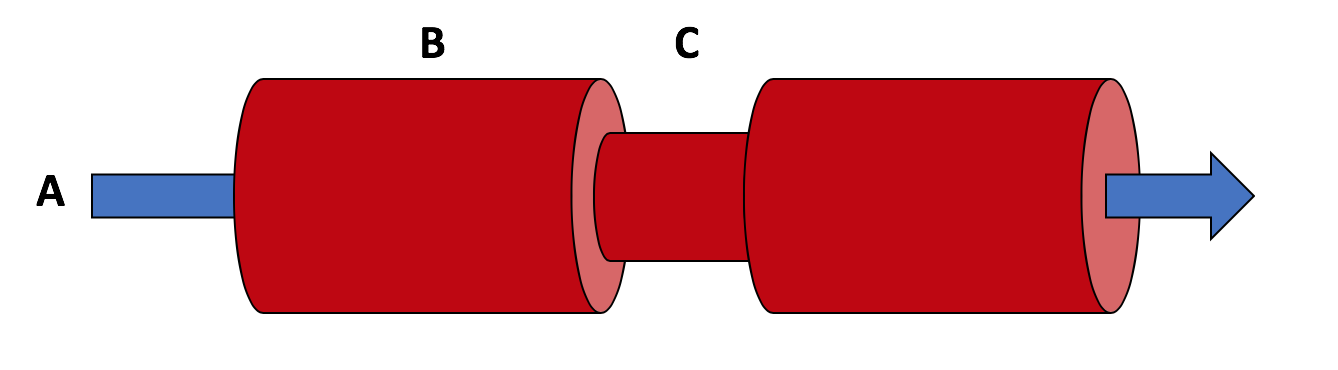
\includegraphics[scale=0.3]{DavidPineiro/stenosis_vein.png}
\centering
\caption{Example artery stenosis we simulate on this report. (A) corresponds to an arrow symbolizing the flow of blood through a vein, (B) demonstrates the normal size of the artery, and (C) highlights the stenosis, a part of the artery which is constricted.}
\label{fig:stenosis_example}
\end{figure}

\subsection{Lattice-Boltzmann Method}
The Lattice-Boltzmann method (LBM) was a natural deduction from Ludwig Boltzmann’s kinetic theory of gases. The method fundamentally understands liquids and gases as a collection of particles undergoing random motions. These particles exchange momentum through particle streaming and inelastic collisions. LBM reduces Boltzmann’s gas dynamics by decreasing the number of particles and confining them to a lattice. In the case of a two dimensional model, particles are restricted to stream in nine directions, including the one for staying in place. This report further delves into the LBM on the section regarding the numerical methods utilized. 


Numerically solving the Boltzmann equation has advantages over numerically solving the Navier-Stokes equations. LBM allows the computation to neglect the nonlinear term, further reducing the amount of computation needed. The method further allows parallelization, which we take advantage of to speed up computation in GPUs and CPUs. LBM remains an upcoming simulation technique for modelling complex fluid systems. LBM has especially gained traction from computational physicists who are able to simulate dynamic problems which would otherwise take larger amounts of time.  

\section{Description of Code}
We used various methods in order to simulate the drug being dissipated through the artery stenosis. 

We first created the shape of the artery using a Python package contained in the file ShapePainter.py which allows us to specify the shape of the vein. This file creates a skeletal mapping of the lattice which is later interpreted by MUPHY another package performing the simulation. ShapePainter.py a .hdr file, which contains the mesh header, a .dat file which details information regarding the mesh nodes, and a .ios file which corresponds to the inlet and outlet boundary conditions which are specified in this file. 

These output files are then interpreted by another package called MUPHY. This package works well for complex and deformed physiological geometries such as veins and arteries, and can cover various
space/time scales with multi-resolution, often useful for physical systems with various scopes. MUPHY is used via MagicUniverse which instantiates a MagicBegins() object that creates an environment for where the LBM computation will take place. There, various fluid objects can be created with specific properties regarding their viscosity among others. 

\section{Numerical Methods Utilized}
The central idea of LBM is to discretize the distribution function $f(\mathbf{x},\mathbf{\xi}, t)$ in the Boltzmann equation. The discretization of the real space naturally gives rise to a squared lattice. The velocity distribution under equilibrium is centered, thus the corresponding discretization can be done by sampling the velocities around that center. In specific, it samples the velocities connecting neighboring sites in the lattice. The discretized  distribution function, also known as the population, becomes $f_i(\mathbf{x}, t)$, with $i$ running over all sampled velocities (denoted as $\mathbf{c}_i$), and $\mathbf{x}$ and $t$ taking over a discrete mesh of spacetime. The macroscopic fields such as the density field and the velocity field are represented by
\begin{align}
    \rho=\sum_if_i(\mathbf{x},t),\quad
    \rho\mathbf{u}=\sum_i\mathbf{c}_if_i(\mathbf{x},t).
\end{align}

The lattice Boltzmann equation with BGK collision operator (LBGK), is
\begin{align}
    f_i(\mathbf{x}+\mathbf{c}_i\Delta t, t+\Delta t)
        =f_i(\mathbf{x}, t)-\frac{\Delta t}{\tau}
         \left(f_i(\mathbf{x}, t) - f_i^\mathrm{eq}(\mathbf{x}, t)\right),
    \label{eqn:lbe}
\end{align}
where the equilibrium population is expanded to the second order
\begin{align}
    f_i^\mathrm{eq}(\mathbf{x}, t)=w_i\rho\left(
        1+\frac{\mathbf{u}\cdot\mathbf{c}_s}{c_s^2}
        +\frac{(\mathbf{u}\cdot\mathbf{c}_s)^2}{2c_s^4}
        -\frac{\mathbf{u}\cdot\mathbf{u}}{2c_s^2}
        \right), 
\end{align}
and viscosity is involved as
\begin{align}
    \nu=c_s^2(\tau-\frac{\Delta t}{2}).
\end{align}
The problem is solved by directly updating the population through Eq. (\ref{eqn:lbe}). 

In our problem, the blood and the drug are treated as two  fluids, each follows a set of LBGK. The blood dynamics is independent, and the drug takes the blood velocity as imposed.

\section{Simulation Parameters}
The geometry of the vessel with stenosis, as well as the initial position of the bolus, is schematically displayed in Figure \ref{fig:stenosis}. The vessel has raidus $R$ and length $L$. The stenosis is located at $A$ with width $S$ and remaining gap $G$. A bolus with width $W$ and the same radius as the vessel is placed at position $d$ at the initial time point. We further constrain these geometric parameters as follows
\begin{align}
    R&=L/20,\\
    d&=L/4,~W=L/20,\\
    A&=L/2,~S=L/10,~G=L/40.\\
\end{align}
\begin{figure}[htbp]
    \centering
    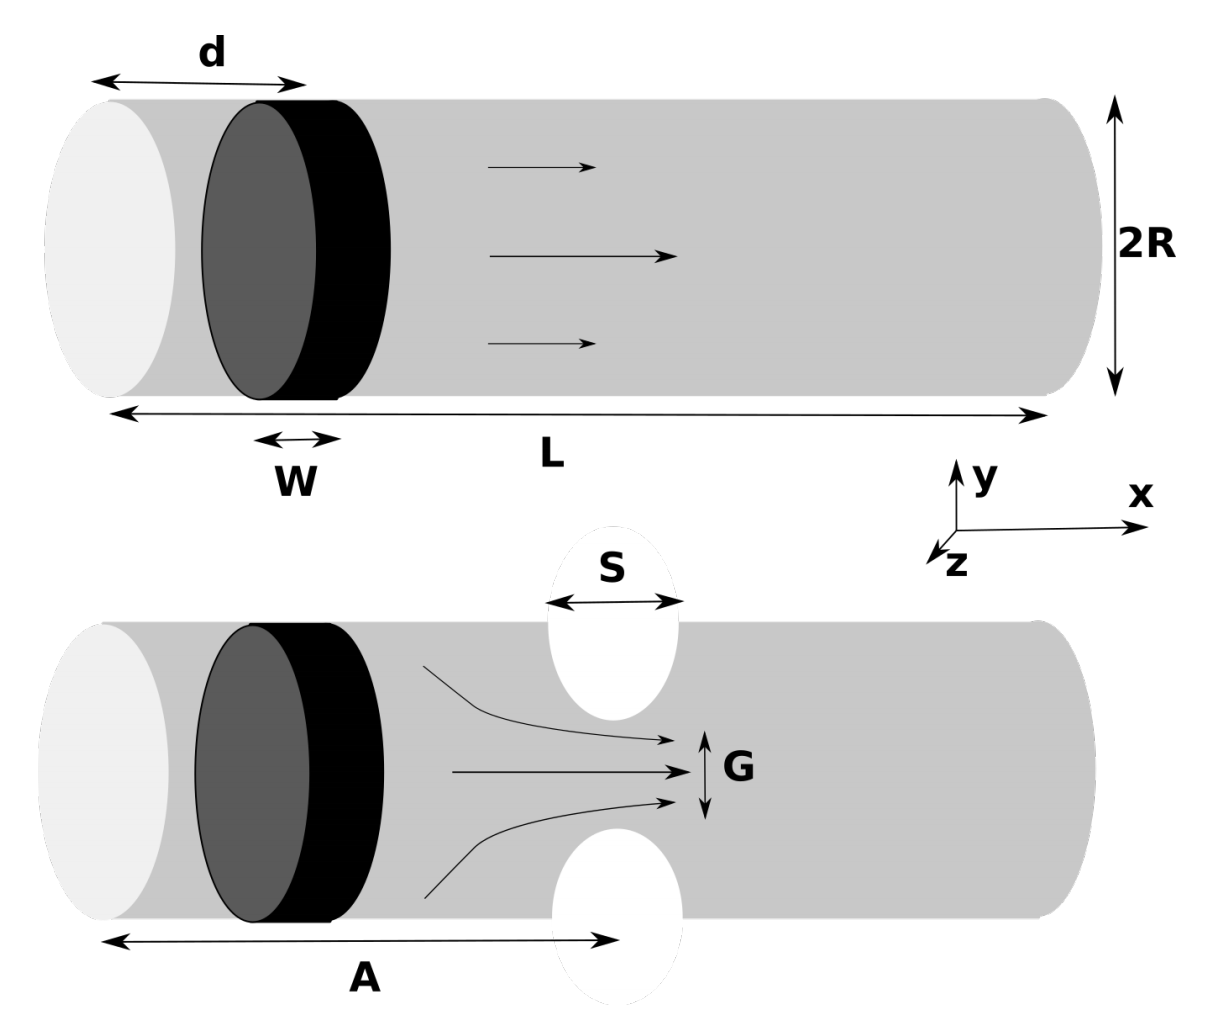
\includegraphics[width=0.6\textwidth]{YiqiXie/stenosis.png}
    \caption{Schematic setup of the problem.}
    \label{fig:stenosis}
\end{figure}

The blood vessel is treated as an impenetrable no-slip boundary. The left end of the vessel is the inlet applied with a driving blood flow
\begin{align}
    u_i(t)=\frac{\bar{u}}{2}\big(1+\cos(2\pi t/T)\big), 
\end{align}
where $T$ is the period of heartbeat. The right end is the outlet applied with fixed pressure (taken as 0 in the simulation). The initial drug concentration in the bolus is high as $c_0$. The boundary condition for the drug concentration is low as $c_1$ at both ends of the vessel. 

The values taken for the parameters are listed in Table \ref{tab:para_physprop}. The geometric scale of the system ($R$), as well as the drug diffusivity ($D$), is tuned to achieve different characteristic numbers, $Re$ and $Pe$. The relationships are
\begin{align}
    Re&=2\bar{u}R/\nu \\
    Pe&=\bar{u}R/D
\end{align}
The simulations are supposed to run through a total physical time of $4T$, with the first $1T$ used to stabilize the blood flow. However, because of the time limit of the project and possible errors from the HPC platform and the MUPHY code, some of the simulations are terminated before $4T$ is arrived. The detailed specifications of each simulation are listed in Table \ref{tab:sim_spec}.
\begin{table}[htbp]
    \centering
    \begin{tabular}{cc}
        \toprule
        Parameter & Value \\
        \midrule
        $\nu$ & 0.1 \\
        $\bar{u}$ & 0.01 \\
        $c_0$ & 1 \\
        $c_1$ & 0.01 \\
        $T$ & $10^6$ \\
        $R$ & (tuned) \\
        $D$ & (tuned) \\
        \bottomrule
    \end{tabular}
    \caption{Parameters of the physical system.}
    \label{tab:para_physprop}
\end{table}

\begin{table}[htbp]
    \centering
    \begin{tabular}{cc|cc|ccc}
        \toprule
         $Re$ & $Pe$ & $R$ & $D$ & Cores & Decomp. & Final Time Step \\
        \hline
         5  & 1.5 & 25 & 0.167 & 128 & $1\times1\times128$ & $4.0\times10^6$ \\
         5  & 3   & 25 & 0.083 & 128 & $1\times1\times128$ & $3.0\times10^6$ \\
         10 & 1.5 & 50 & 0.333 & 512 & $2\times2\times128$ & $1.3\times10^6$ \\
         10 & 3   & 50 & 0.167 & 512 &
         $2\times2\times128$ & $1.1\times10^6$ \\
        \bottomrule
    \end{tabular}
    \caption{Simulation specifications. }
    \label{tab:sim_spec}
\end{table}

% \pagebreak  % put a pagebreak to ensure the correct formatting of the result section.
\clearpage
\section{Results}
\graphicspath{ {./JiaweiZhuang/img/} }

\subsection{Basic behavior of blood and drug fields}

We first describe the basic behavior of blood and drug fields during the simulation. The $Re=5, Pe=1$ case is used as the major example, as the different cases show similar overall behavior (just with different magnitudes and diffusion rates). The effect of $Re$ and $Pe$ is discussed in the next section.

Because the x and y directions are symmetric in our problem, we can visualize the 3-D blood vessel using 2-D "longitudinal cuts", by slicing over the middle point of x-axis and only plot the y-z cross section. 

Fig \ref{fig:density} shows the blood density. The density oscillate according two the heart beat (please refer to the animation in the slides). Here we only plot two steps with the middle and the highest value. Because of the inlet flow from the left, density is high on the left and low on the right. The major transition happens in the middle stenotic/narrow region, which shows large density gradient.

\begin{figure}[H]
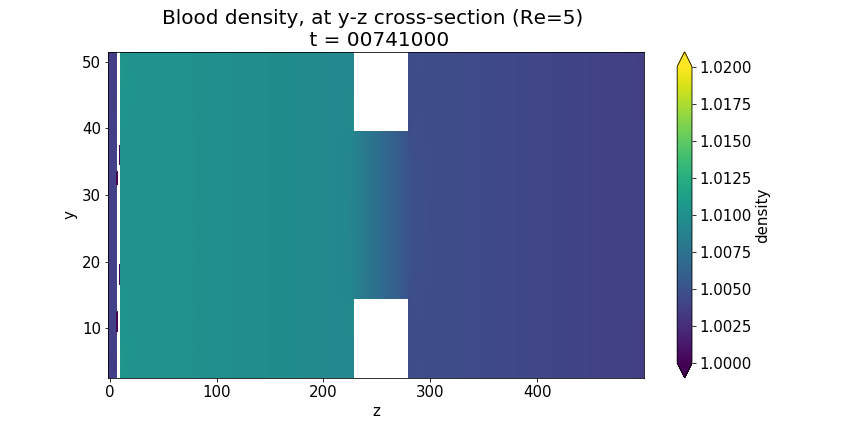
\includegraphics[scale=0.3]{cross_section/density_148}
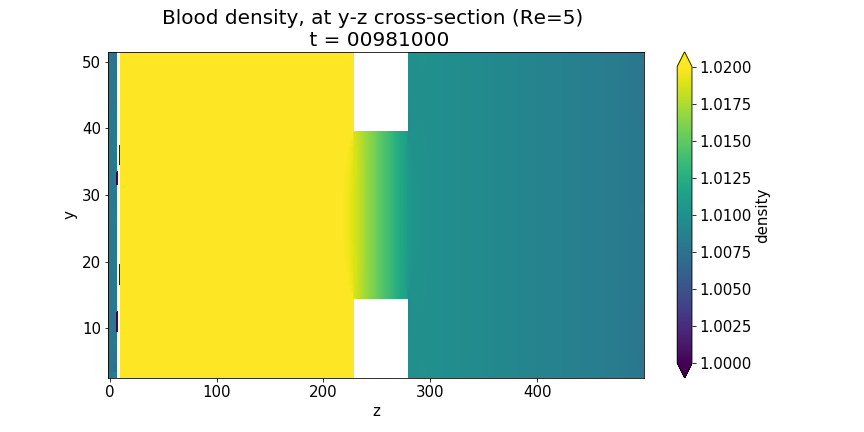
\includegraphics[scale=0.3]{cross_section/density_196}
\centering
\caption{Blood density at 2-D longitudinal cuts (Re=5, Pe=1 case).}
\label{fig:density}
\end{figure}

We then perform the Schlieren visualization on the density field, using the formula:

\begin{align}
Sch = exp(-k\frac{|\nabla T|}{max(|\nabla T|)})
\end{align}

where $T$ is the original field. Here it is the blood density.

Fig \ref{fig:sch} shows the Schlieren field with $k=20$. We don't see interesting patterns due to the lack of spatial gradient. Unlike Module 1’s Rayleigh-Benard Convection with highly complex patterns, in this blood flow case there is little spatial variations and the flows are highly laminar. The middle stenotic region has the highest Schlieren value, corresponding to the high gradient here.

\begin{figure}[H]
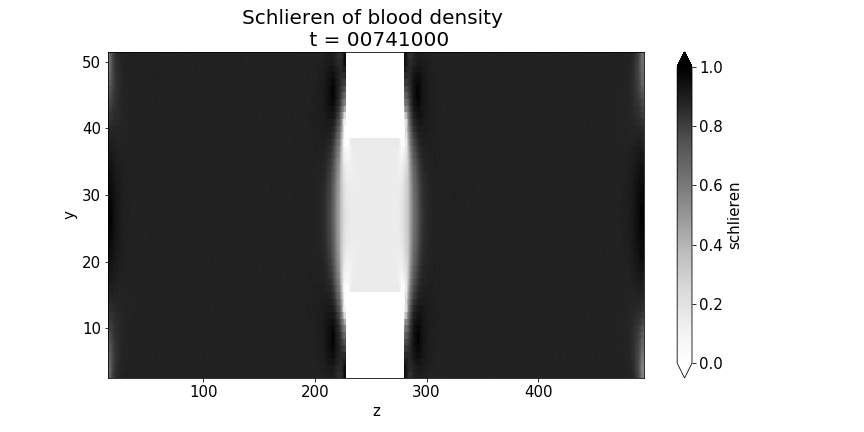
\includegraphics[scale=0.3]{cross_section/schlieren_148}
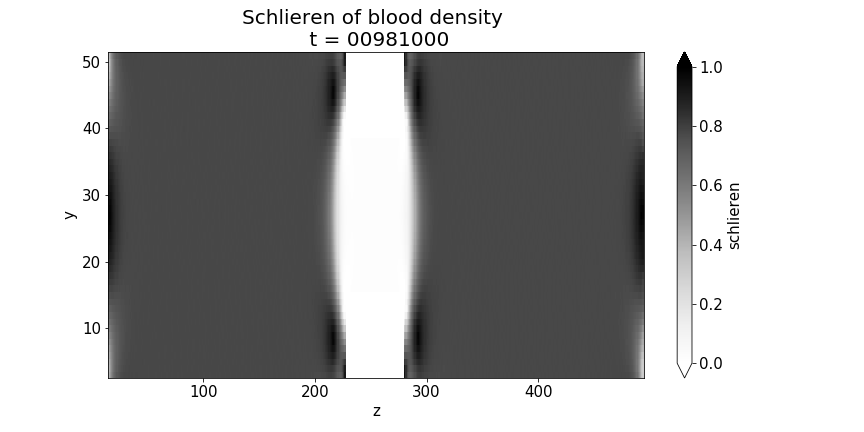
\includegraphics[scale=0.3]{cross_section/schlieren_196}
\centering
\caption{Schlieren visualization of blood density at 2-D longitudinal cuts (Re=5, Pe=1 case).}
\label{fig:sch}
\end{figure}

We then turn to the blood velocity. Fig \ref{fig:uz} shows the velocity magnitude and Fig \ref{fig:streamline} shows the streamline. Velocity also oscillates following the heart beat.
The stenotic region has the highest velocity, consistent with the continuity equation. The streamlines follow the the blood vessel shape.

\begin{figure}[H]
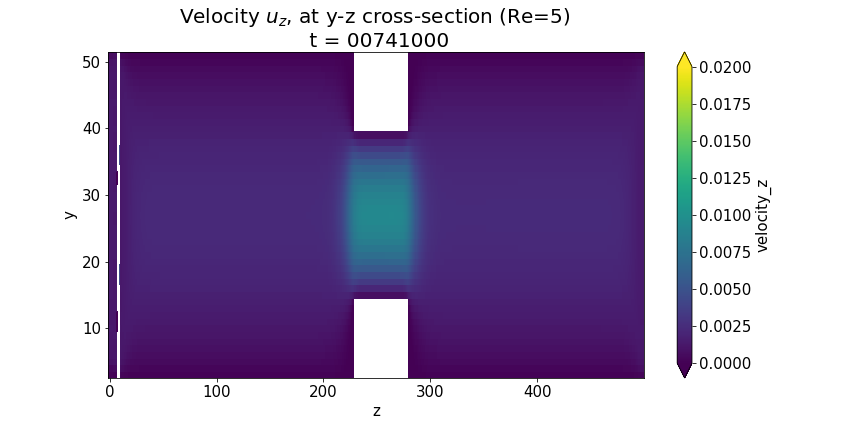
\includegraphics[scale=0.3]{cross_section/uz_148}
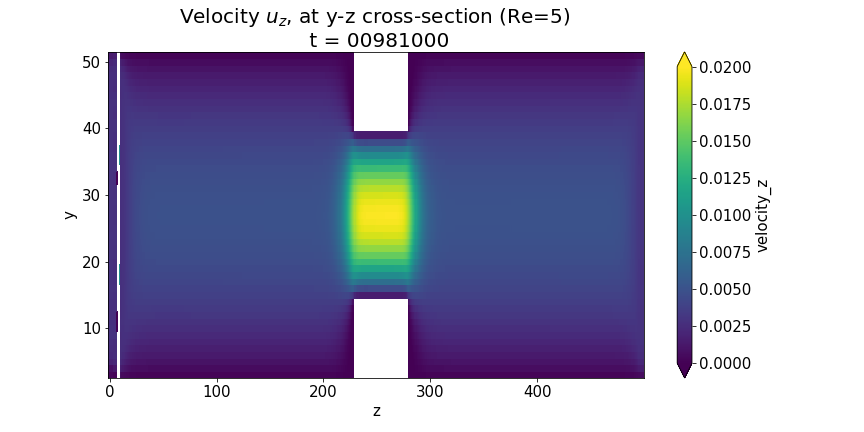
\includegraphics[scale=0.3]{cross_section/uz_196}
\centering
\caption{Blood velocity at 2-D longitudinal cuts (Re=5, Pe=1 case). Plotted is the z-component. The x, y components are orders of magnitude smaller and contribute little to the total magnitude.}
\label{fig:uz}
\end{figure}


\begin{figure}[H]
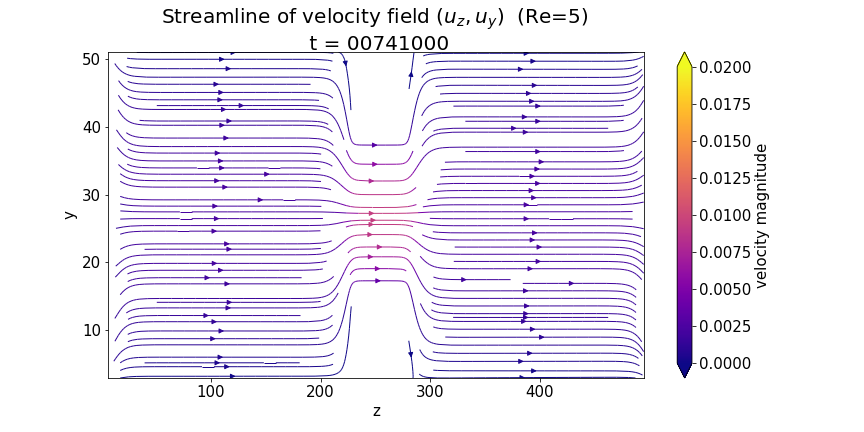
\includegraphics[scale=0.3]{cross_section/streamline_148}
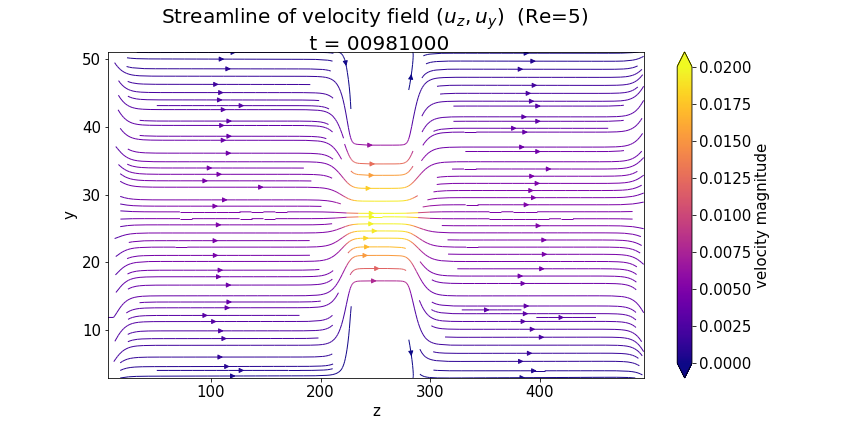
\includegraphics[scale=0.3]{cross_section/streamline_196}
\centering
\caption{Streamline of blood velocity at 2-D longitudinal cuts (Re=5, Pe=1 case), colorred with velocity magnitude.}
\label{fig:streamline}
\end{figure}

Last, we visualize the diffusion of the drug, in Fig \ref{fig:drug}. The drug is released at $1/4$ of total simulation time ($1 \times 10^6$ steps). It then gets diffused very quickly and pushed rightward following the flow direction. Just after 20,000 steps ($0.5\%$ of total simulation time), the main body of the drug field enters the stenotic region.

\begin{figure}[H]
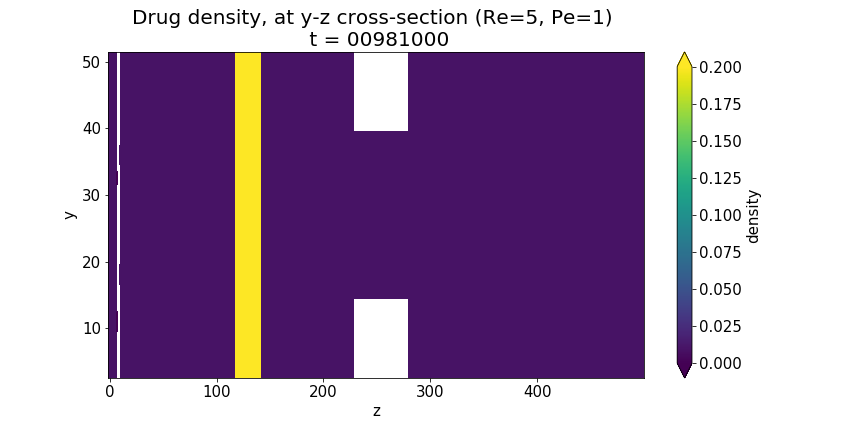
\includegraphics[scale=0.3]{cross_section/drug_196}
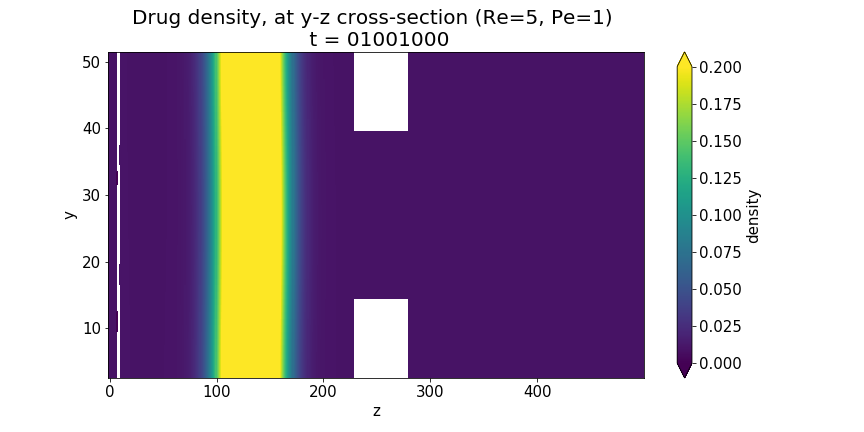
\includegraphics[scale=0.3]{cross_section/drug_200}
\centering
\phantomcaption
\end{figure}

\begin{figure}[H]\ContinuedFloat
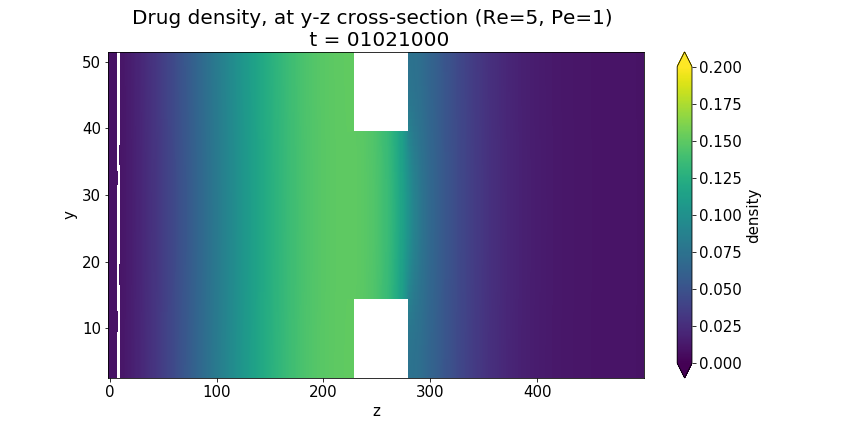
\includegraphics[scale=0.3]{cross_section/drug_204}
\centering
\caption{Drug density at 2-D longitudinal cuts (Re=5, Pe=1 case)}
\label{fig:drug}
\end{figure}

\subsection{Effect of Peclet number and Reynolds numbers on drug efficacy}

To better show the drug spread over time, we plot the drug profile averaged over the cross-section (x, y directions). Fig \ref{fig:drug_profile} shows the profiles for Re5Pe1 and Re5Pe3 cases. A larger Peclet number leads to slower diffusion of drug, as expected (due to higher viscosity). The profile has minor discontinuities at the entries of the stenotic region, due to the abrupt change in the denominator (cross-section size) when computing the mean.

\begin{figure}[H]\ContinuedFloat
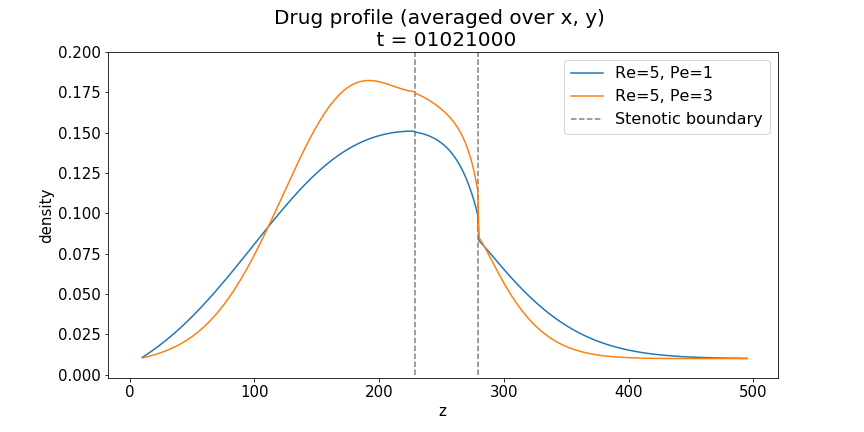
\includegraphics[scale=0.4]{drug_profile/drug_profile_204}
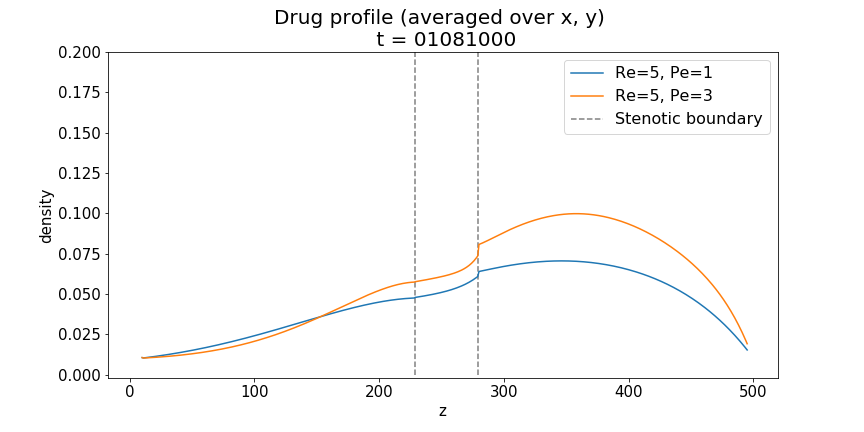
\includegraphics[scale=0.4]{drug_profile/drug_profile_216}
\centering
\caption{Drug profile averaged over x-y cross-section, for Re5Pe1 and Re5Pe3 cases.}
\label{fig:drug_profile}
\end{figure}

To show the drug efficacy, we compute the integral of drug density (i.e. drug mass) over the stenotic region, as plotted in Fig \ref{fig:drug_efficacy}. After the drug lease at $step = 1 \times 10^6$, it diffuses very quickly, in less than $5 \times 10^5$ steps ($1/8$ of the total time). Again, a large Peclet number leads to slower diffusion and thus higher drug efficacy. For the large Reynold number case (Re10), the drug mass is 8 times higher, proportional to the increased domain size; but the time evolution has a similar trend as Re5 cases.

\begin{figure}[H]
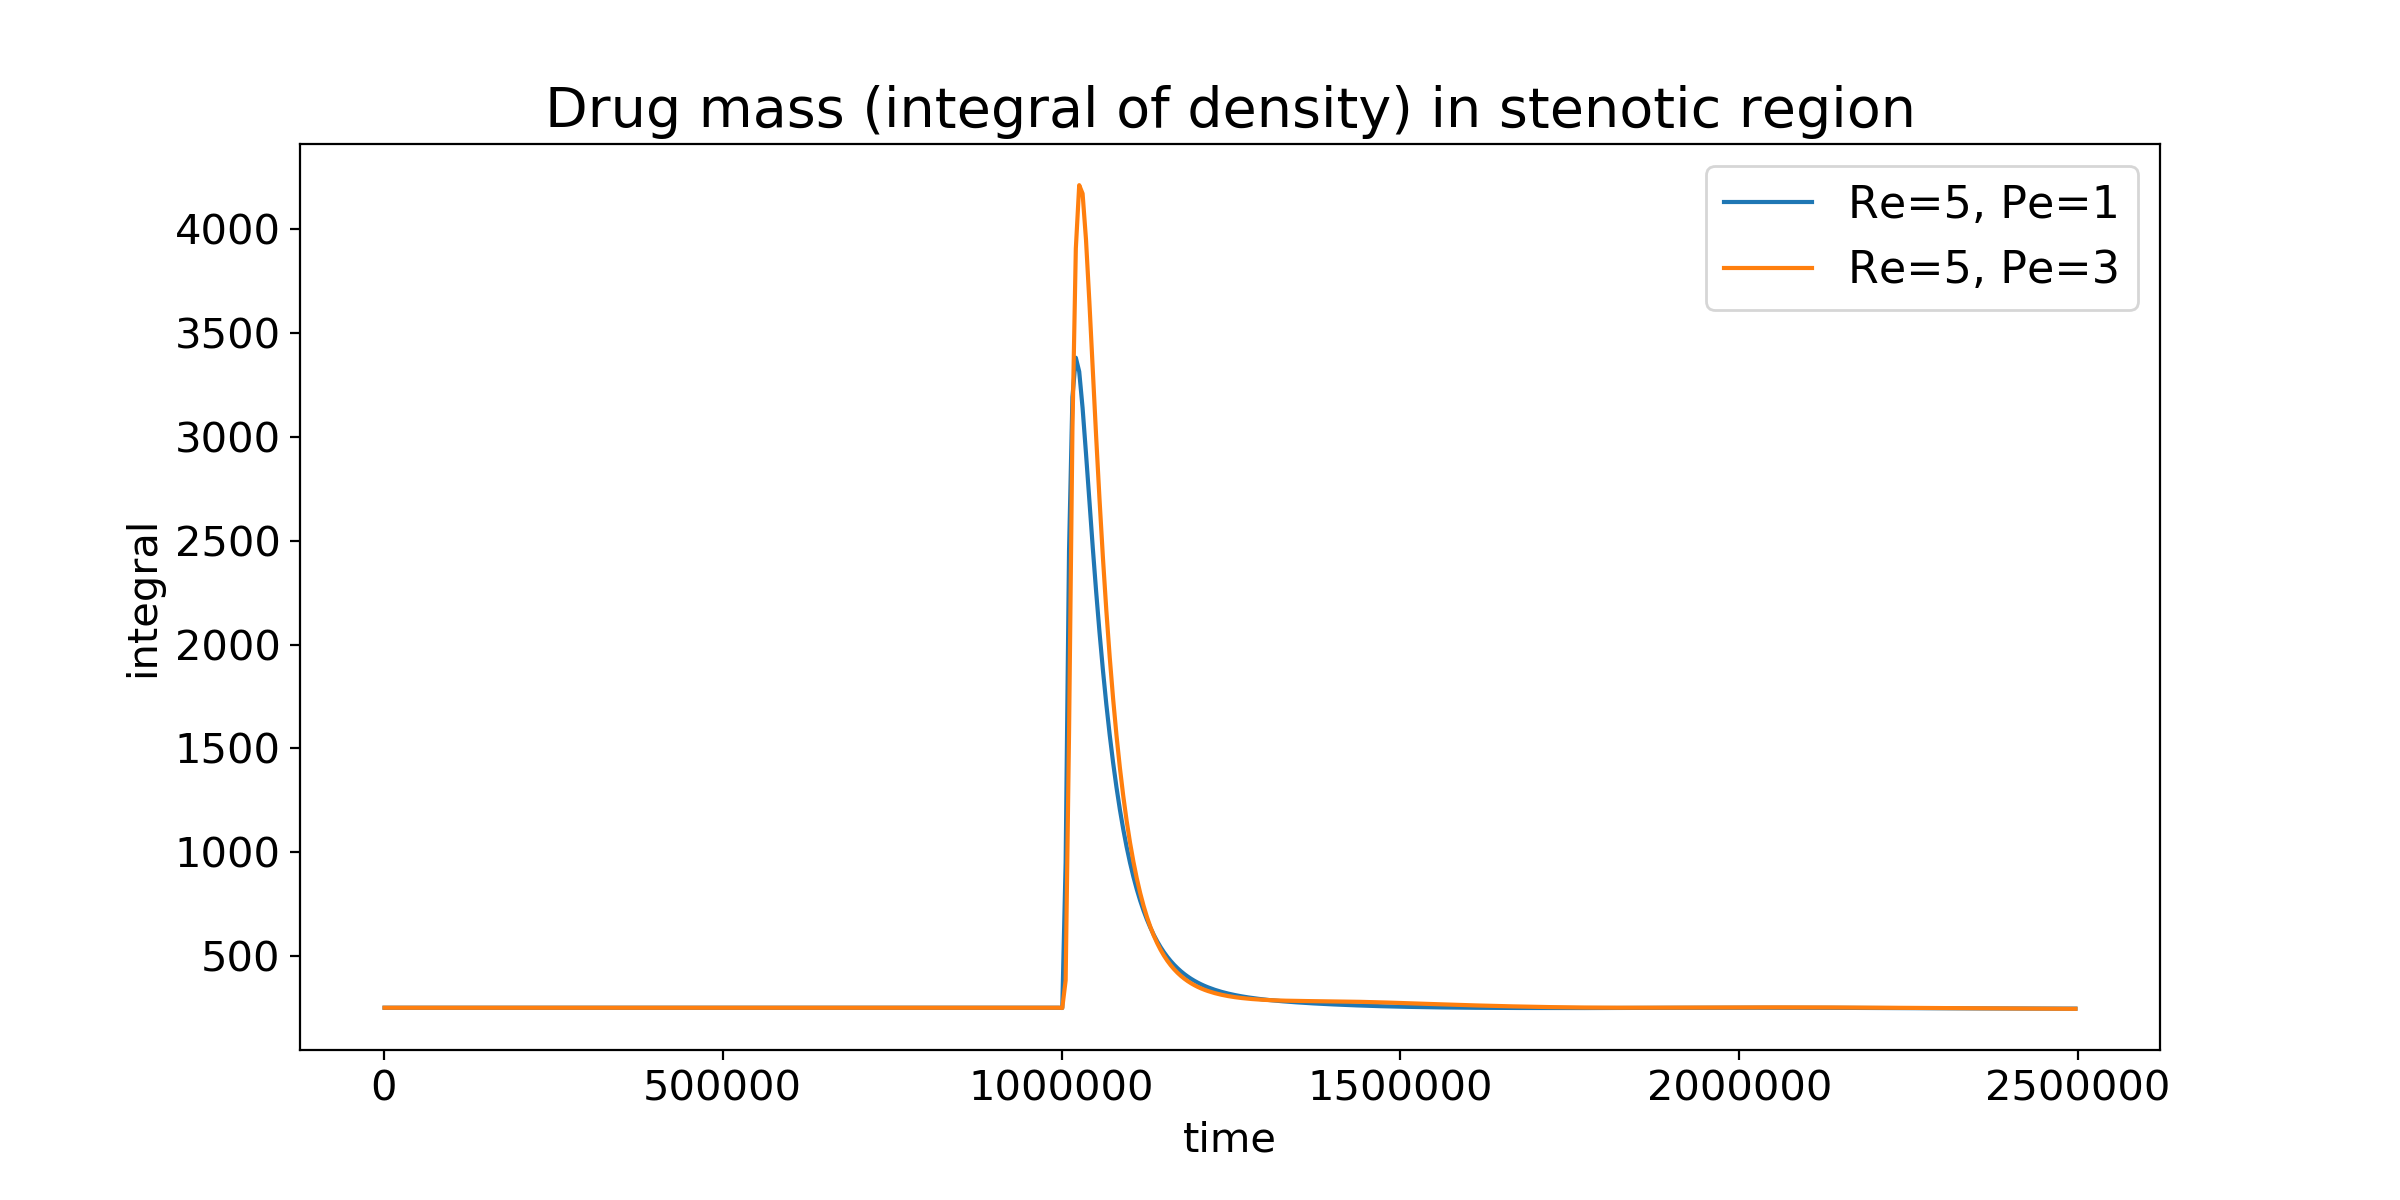
\includegraphics[scale=0.4]{drug_efficacy/drug_integral_re5_fulltime.png}
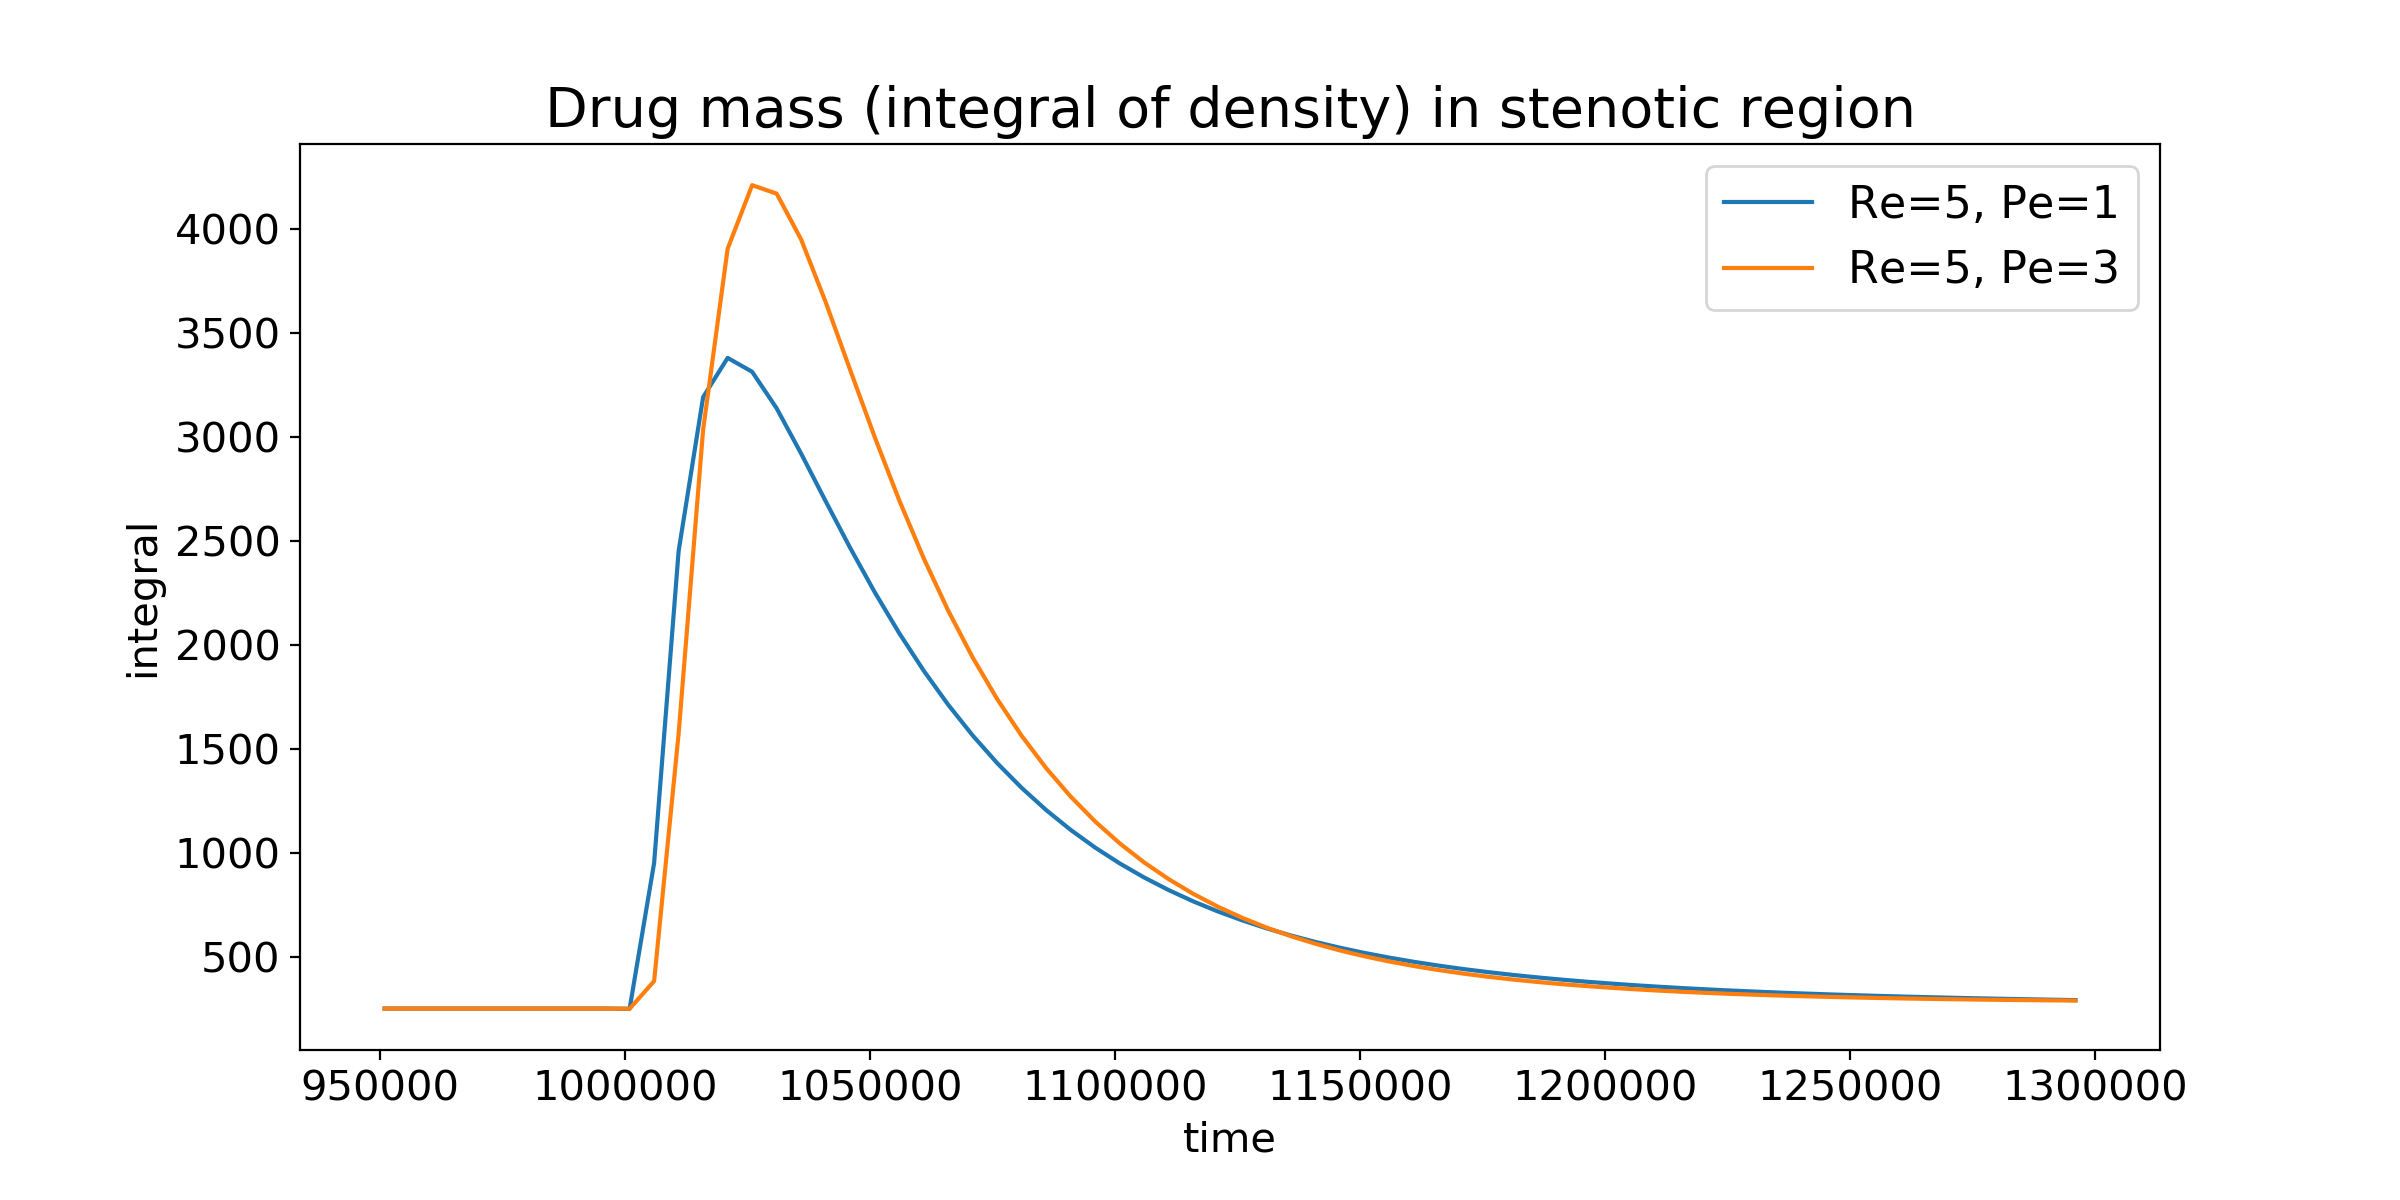
\includegraphics[scale=0.4]{drug_efficacy/drug_integral_re5_hightime.png}
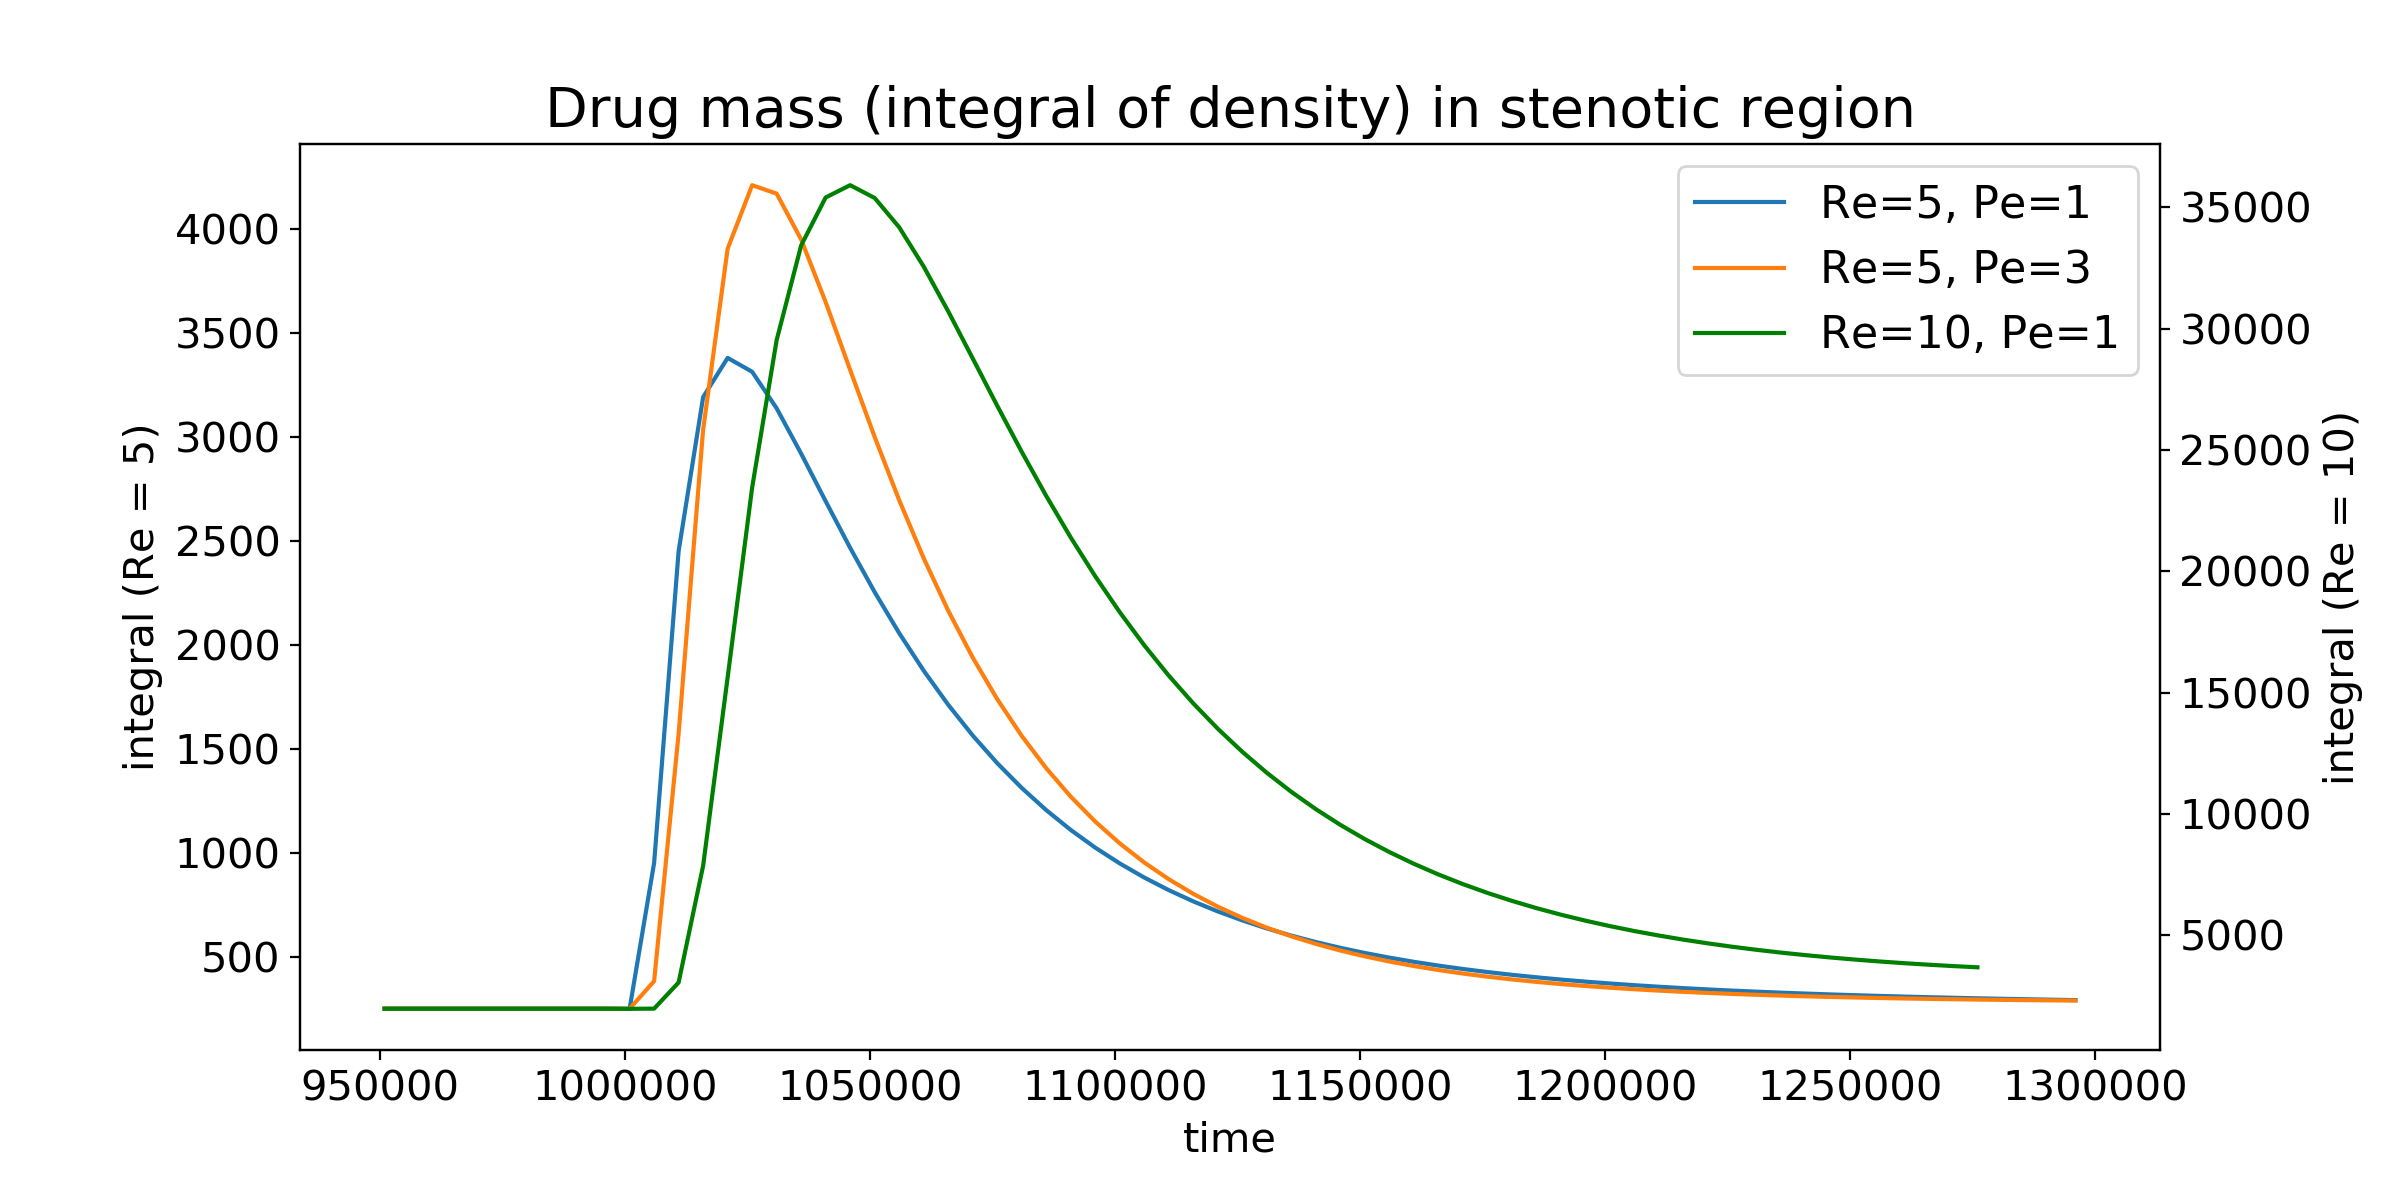
\includegraphics[scale=0.4]{drug_efficacy/drug_integral_re5and10_hightime.png}
\centering
\caption{Drug efficacy (integral over narrow region. The first figure shows the full time axis. The second figure is the zoomed-in version, highlighting the period with high drug density. The third figures adds the Re10 case on a twin y-axis.}
\label{fig:drug_efficacy}
\end{figure}

\subsection{3-D streamline visualization}

A particularly interesting phenomenon can be shown in 3D streamline visualization. We use ParaView StreamTracer to visualize the blood streamline at a single time slice, as shown in Fig \ref{fig:streamline_demo}. Different time slices have similar streamlines although different velocity magnitudes. Near the entries of the stenotic region, there are many small whirls, forming a big circle.

\begin{figure}[H]
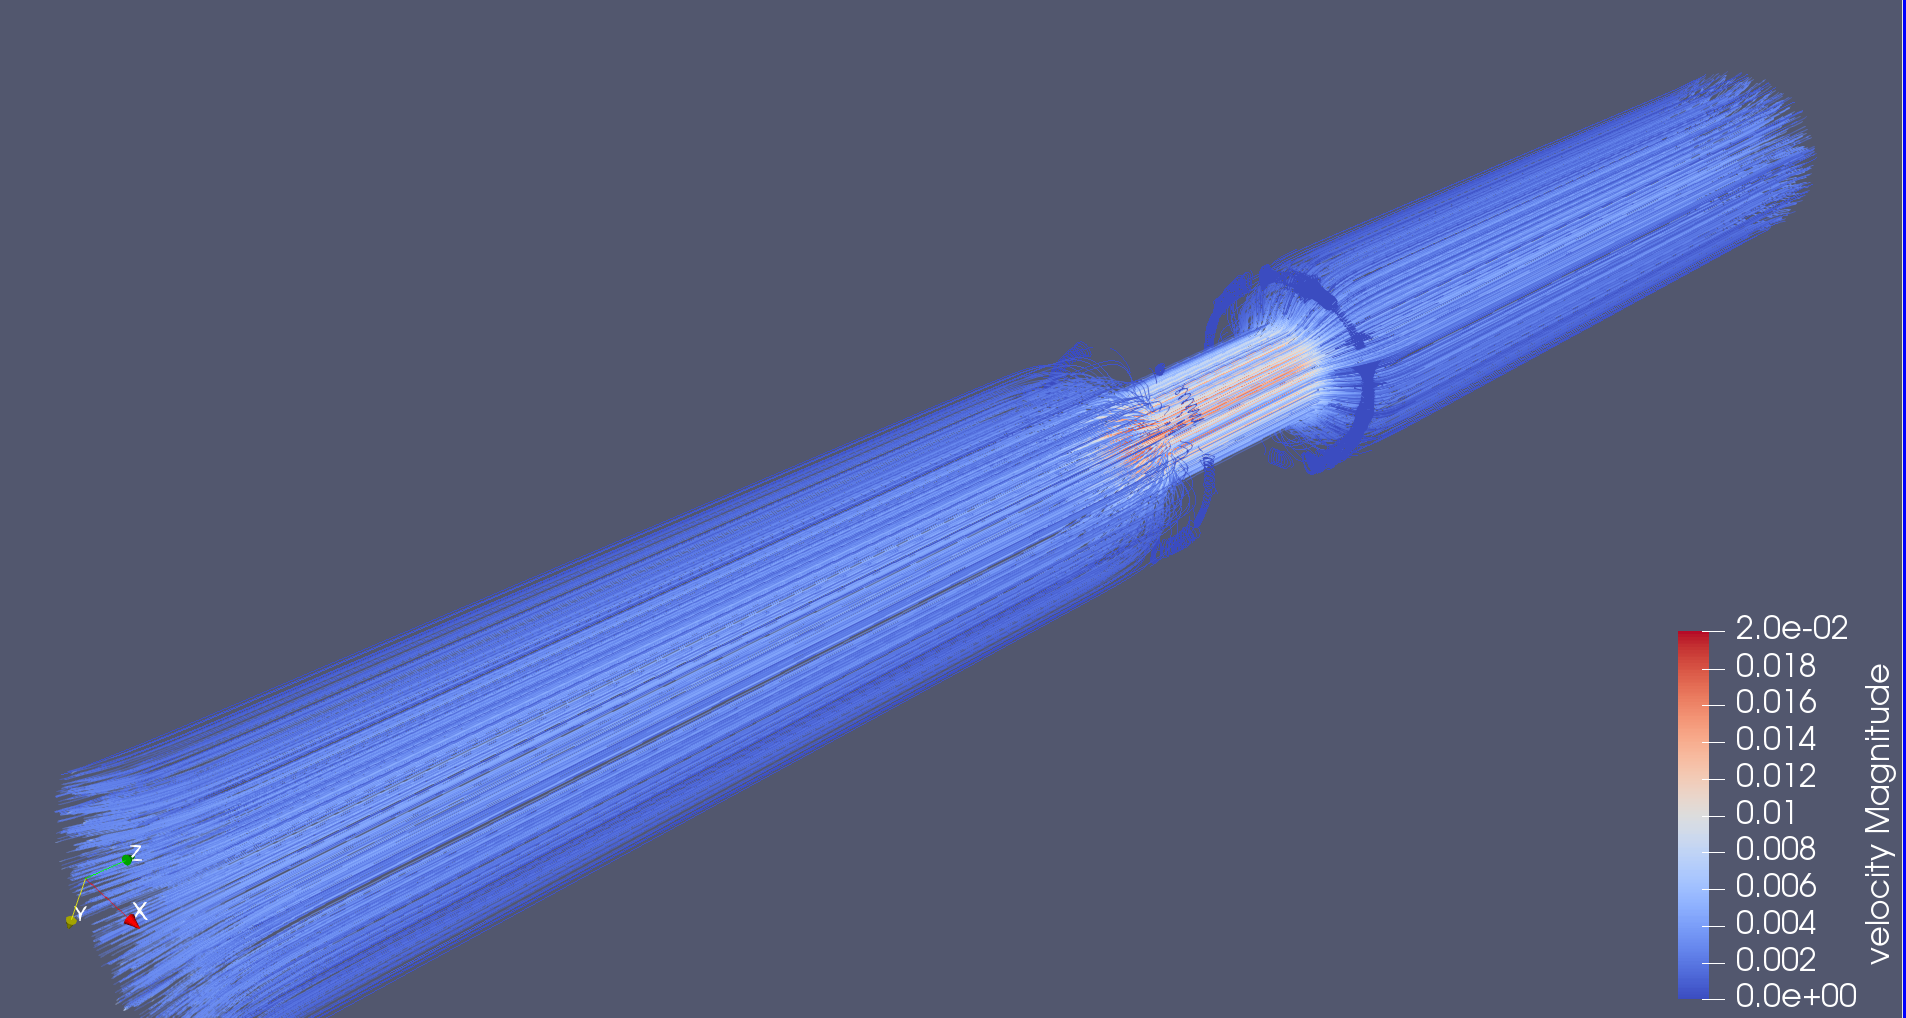
\includegraphics[scale=0.44]{streamline_3d/streamline_demo.png}
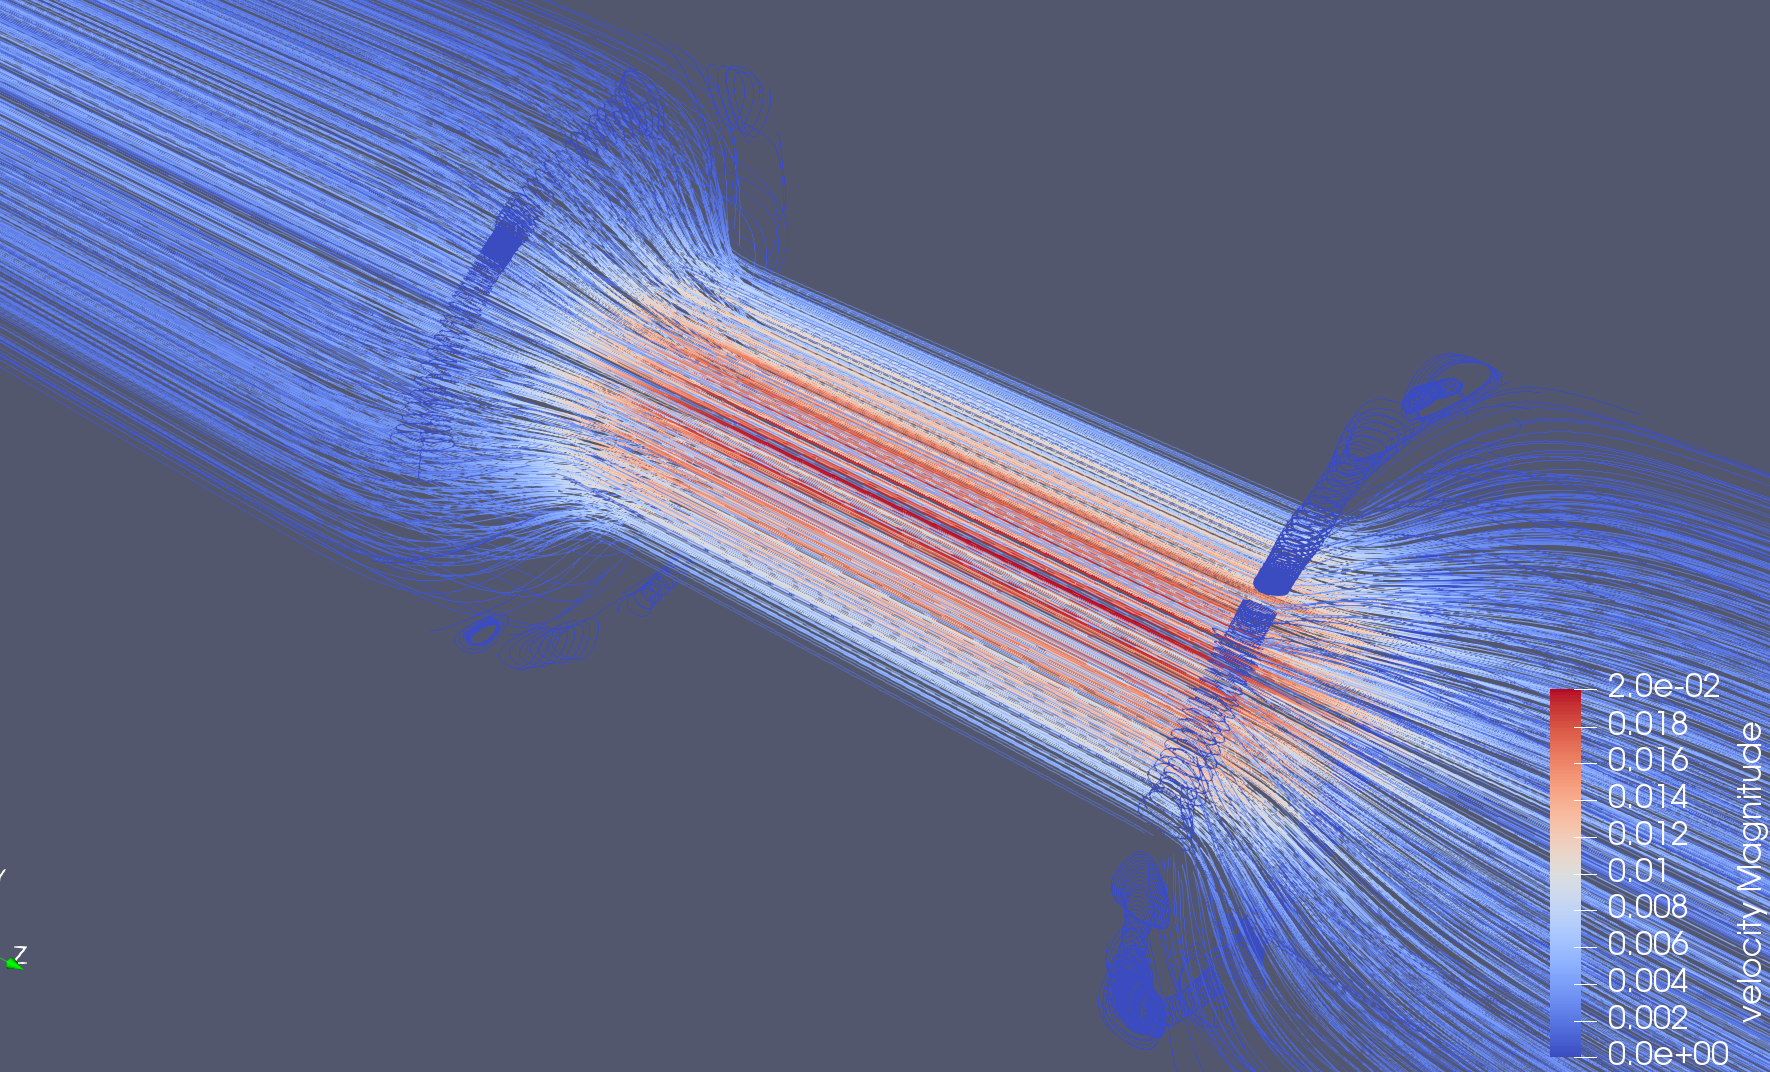
\includegraphics[scale=0.48]{streamline_3d/small_whirls_demo.png}
\caption{3-D Streamlines generated by ParaView. Colors are velocity magnitudes.}
\label{fig:streamline_demo}
\end{figure}

To further highlight to streamline, we color the lines with streamline types \footnote{https://kitware.github.io/paraview-docs/latest/python/paraview.simple.StreamTracer.html} instead of velocity magnitude, as shown in Fig \ref{fig:streamline_color}. A value of 1 (blue color) means that the streamline exceeds the domain boundary. Most streamlines belong to this case, as they all go from the left inlet to the right outlet. A value of 3 or more (white or red colors) means that streamline terminates due to the violation of some limits such as line length or integration steps. The small whirls belong to this case as they form a closed circle without connecting to external boundaries. Those small whirls occur when the fluid hit the blood vessel boundary and bounce back. 

\begin{figure}[H]
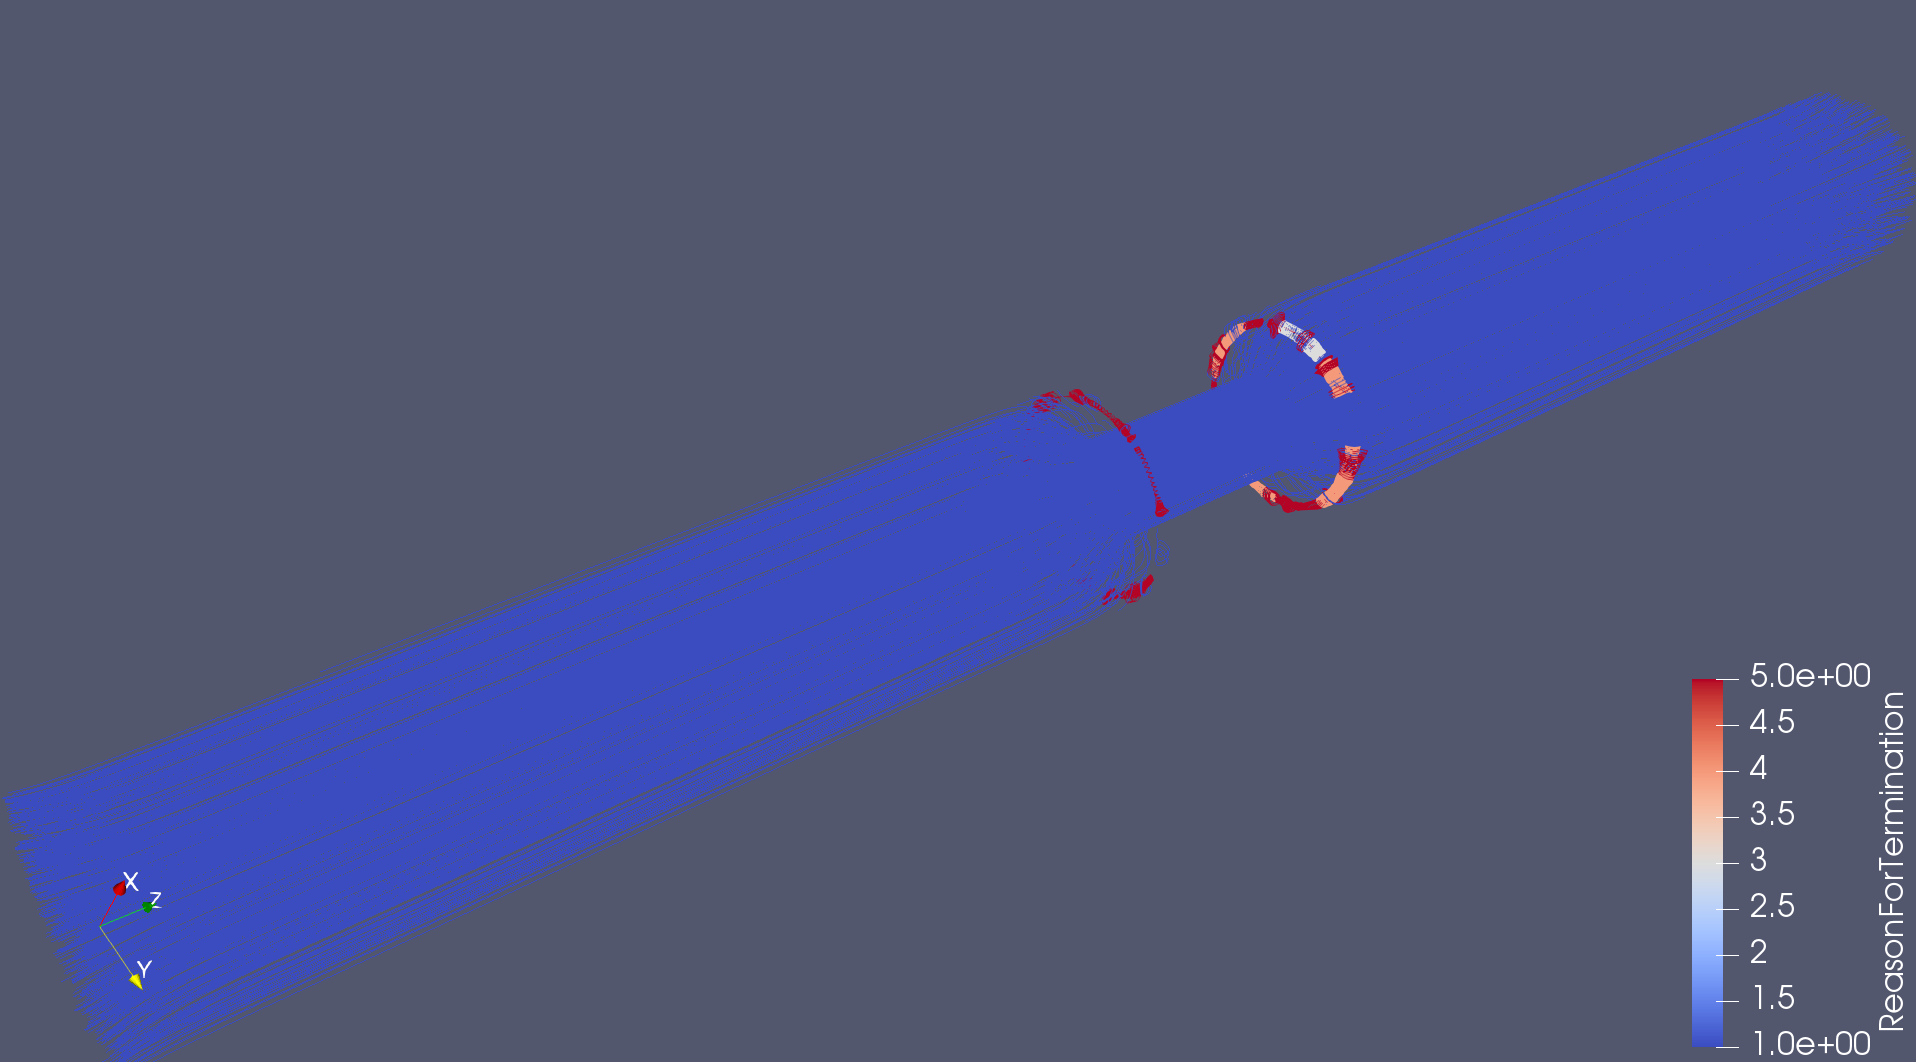
\includegraphics[scale=0.45]{streamline_3d/streamline_color.png}
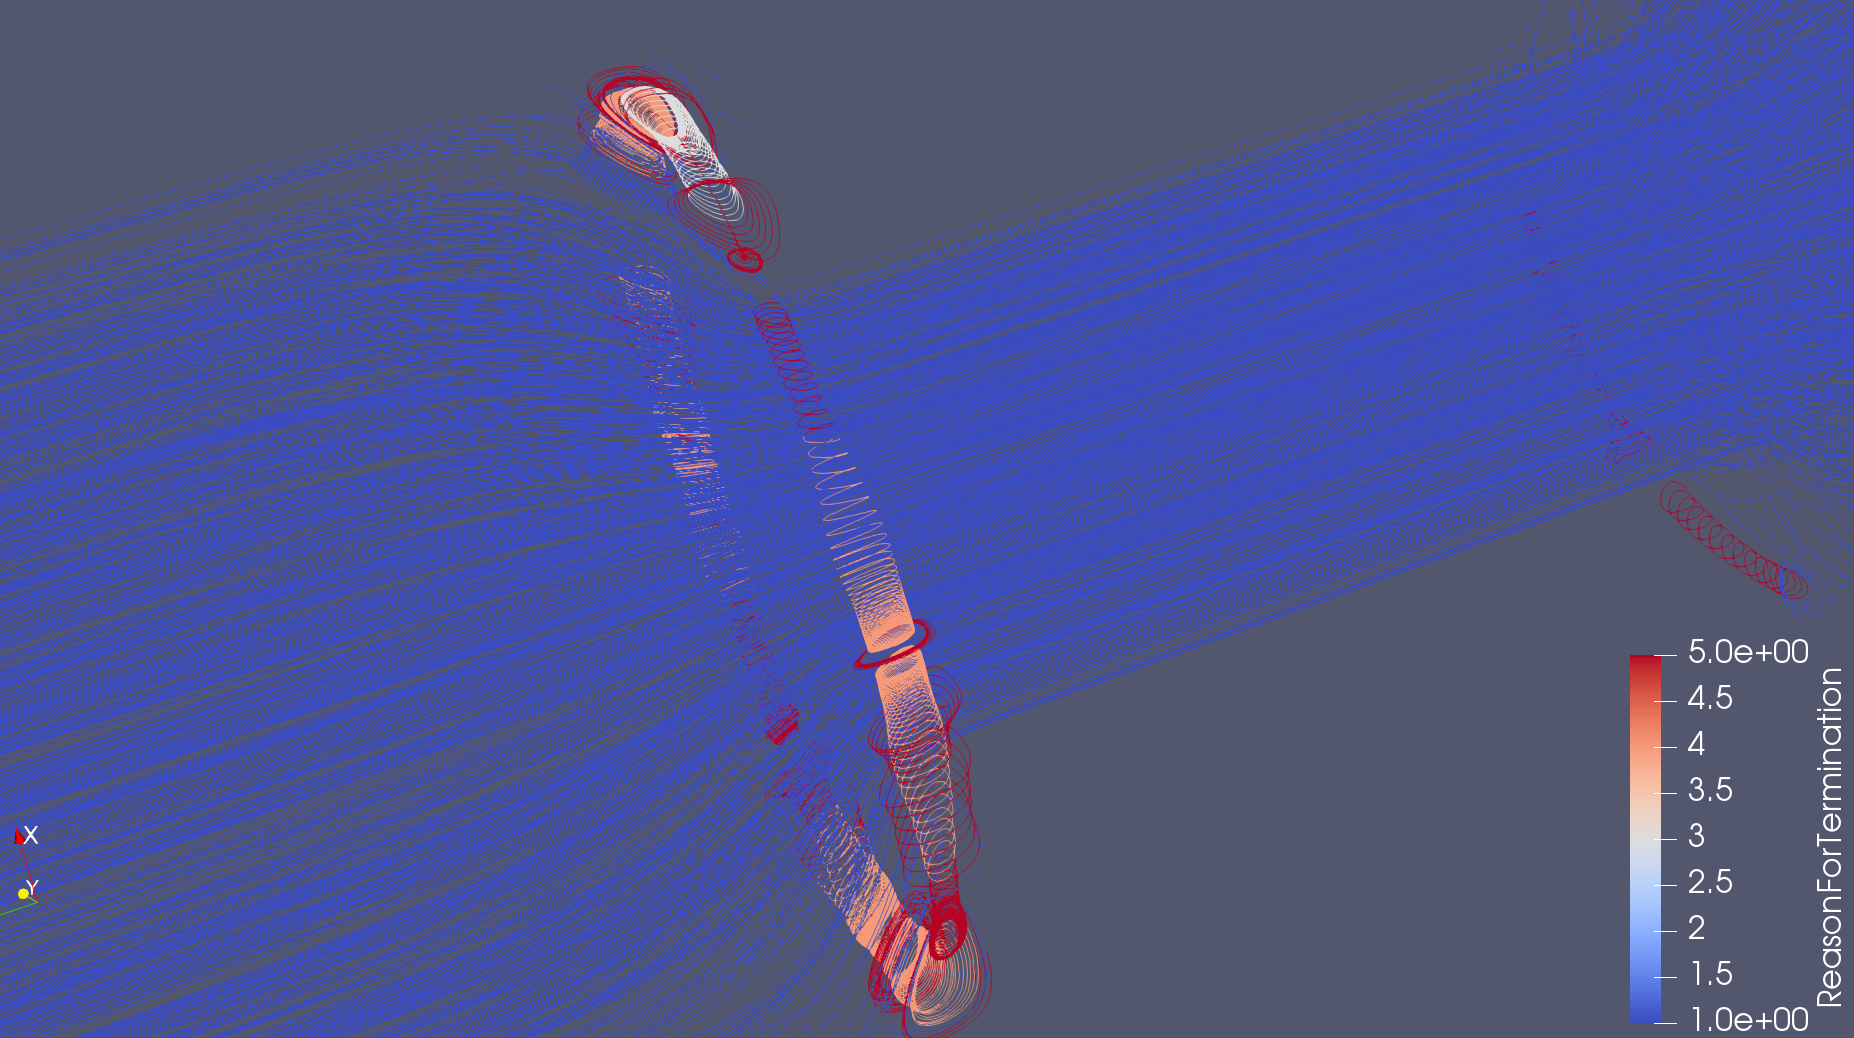
\includegraphics[scale=0.47]{streamline_3d/small_whirls_color.png}
\caption{3-D Streamlines generated by ParaView. Colors are streamline types, to highlight the small whirls.}
\label{fig:streamline_color}
\end{figure}

\subsection{Data post-processing methods and code availability}

The original VTK files generated by Murphy simulations are very big and difficult to analyze. The output frequency is set to every $1000$ steps; with the total $4 \times 10^6$ steps, 4000 output files are generated for each simulation case.

\begin{itemize}
	\item For $Re = 5$ cases, each time step produces $224 MB$ data, leading to $224 MB \times 4000 = 900 GB$ total data.
	\item For $Re = 10$ cases, each time step produces $1753 MB$ data, leading to $1753 MB \times 4000 = 7000 GB$ total data.
\end{itemize}

The file size calculation is available at: JiaweiZhuang/check\_raw\_vtk\_files.ipynb

Considering a typical disk throughput of 500 MB/s, reading 1000 GB data will take 30 minutes. Analyzing such huge data in the real-time is not feasible. 

To efficiently process and visualize the data, we conducted the following steps:

\begin{itemize}
	\item \textbf{Down-sampling}. Because the physical system is changing slowly, with a time scale determined by the heart beat frequency, the original 1000-step output frequency is not necessary. We can still resolve the flow evolution with a 5000-step frequency. This reduces the data size by 5 times.
	\item \textbf{Reorganizing and compressing}. Although our problem is defined on a 3D uniform grid mesh, the VTK files store the data as unstructured meshes. The grid coordinates are unnecessarily repeated for each grid point. By storing the same data as structured 3-D arrays, we removed the redundant grid coordinate information. The 3-D data are then written to NetCDF format, with additional compression. We use vtki (https://github.com/vtkiorg/vtki) to load VTK files in Python, and then use Xarray (https://github.com/pydata/xarray) to write and read NetCDF files. The scripts for this step are JiaweiZhuang/preprocess\_vtk.py and JiaweiZhuang/submit\_preprocess.sh. This step further reduces data size by 10 times. 
	\item \textbf{Out-of-core computing}. Although the final data size is reduced to about 100 GB, it is still much bigger than the CPU memory of a normal laptop, and close to the total memory of a compute node on Odyssey cluster. We use Dask (https://github.com/dask/dask) for out-of-core computation to avoid exhausting the memory. The code for this step is JiaweiZhuang/all\_plots\_for\_report.ipynb
\end{itemize}

Those post-processing optimizations allow us to generate the plots for this report and the presentation in a few hours, instead of many days.


\section{Conclusion and Future Work}
In this work we have studied drug dispersion in a stenotic artery through LBM simulations running on an HPC platform. The physical system is tested with different $Re$ and $Pe$. The result shows that the drug efficacy is higher with both high $Re$ and high $Pe$, which provides important clues for the design of drug releasement in the treatment of the stenosis. Although the $Re=10$ case only run to about 30\% of total simulation and crashed, the drug had already diffused far enough in such a short time, so we can still compute the drug efficacy. Our analysis has also found some interesting fluid behavior in and around the stenotic area. For instance, that area has the highest density gradient and velocity; many small whirls are generated when the blood hit the wall around the narrow. For other areas, the flow is highly laminar, as the Reynolds number is very small compared to that of turbulent flows ($Re>1000$)

Our current simulation geometry applied rectangular stenosis to the artery, which is a rough approximation to the real condition. For future work, one may investigate into the shape effect of the stenosis. In addition, transferring the simulations to distributed GPU architecture may further improve computational performance and help to run more tests within a reasonable period of time. 


\bibliographystyle{unsrt}  
%\bibliography{references}  %%% Remove comment to use the external .bib file (using bibtex).
%%% and comment out the ``thebibliography'' section.


\begin{thebibliography}{1}

% Example:
% \bibitem{kour2014real}
% George Kour and Raid Saabne.
% \newblock Real-time segmentation of on-line handwritten arabic script.
% \newblock In {\em Frontiers in Handwriting Recognition (ICFHR), 2014 14th
%   International Conference on}, pages 417--422. IEEE, 2014.

\bibitem{}
Bernaschi, M., Melchionna, S., Succi, S., Fyta, M., Kaxiras, E., \& Sircar, J. K. (2009). MUPHY: A parallel MUlti PHYsics/scale code for high performance bio-fluidic simulations. Computer Physics Communications, 180(9), 1495-1502.

\end{thebibliography}


\end{document}
